\chapter{Band structure engineering}
\label{chap:methods}
\section*{Chapter description}

In this chapter, the methodology of the results obtained will be described in detail.
Each type of band structure engineering will be covered separately and all important aspects noted.
Each step will be presented one after another.
All results given in part \hyperref[part:III]{\Romanbar{III}} are set exactly in the same order to simplify the analysis of the research result.
Methods are also shown in such sequence that the first is the least invasive, to material structure, type, and each next changes more in former material.
\ornament
\section{Strains}
\label{sect:strain_theory}

In this part of work all calculations were conducted with ABINIT software package.

Applying strains to a material is the easiest way of modifying its physical properties.
In practice, many experimental solutions can be found.
One can apply isotropic (hydrostatic) strains by using diamond anvils or produce biaxial (planar) strains by adsorbing considered material's atoms to the surface of another material with different lattice constant, creating a thin film.
Due to the volume of the base material, the adsorbent will dictate the crystallographic structure, as well as in plane lattice constants, of the film created on the surface.
Such a film can be produced precisely with MBE (molecular beam epitaxy) method.

In this work there were three types of strains considered:
\begin{itemize}
	\item isotropic (hydrostatic)
	\item uniaxial (in line)
	\item biaxial (in plane)
\end{itemize}
Moreover, in the case of non--isotropic strains, the direction of straining is also crucial.
Different type will usually result in various changes in the electronic structure.
To have a full view over straining effect, research must be conducted in every meaningful direction.
However, the choice is strongly dependent on crystal symmetries.
In this work, only the simplest cases were taken under consideration, as a firm base of research, which are pure group IV crystals in diamond structure.
This choice is dictated by the fact that silicon itself crystallizes in a diamond structure under standard conditions, and group IV elements are isovalent to silicon.
That means that all of the technology associated with it should be applicable, too.
In case of diamond structure, the relevant directions of the strains are $[100]$, $[110]$, and $[111]$.
Those three cover all the unique cases, and every possible direction can be represented as a linear combination of the ones named before.
The given directions will be used for all group IV elements in both, uniaxial and biaxial, cases.
The picture \ref{Fig:strain_direction} represents \conv\ of the diamond structure with the straining directions marked.

\begin{figure}[!htbp]
	\centering
	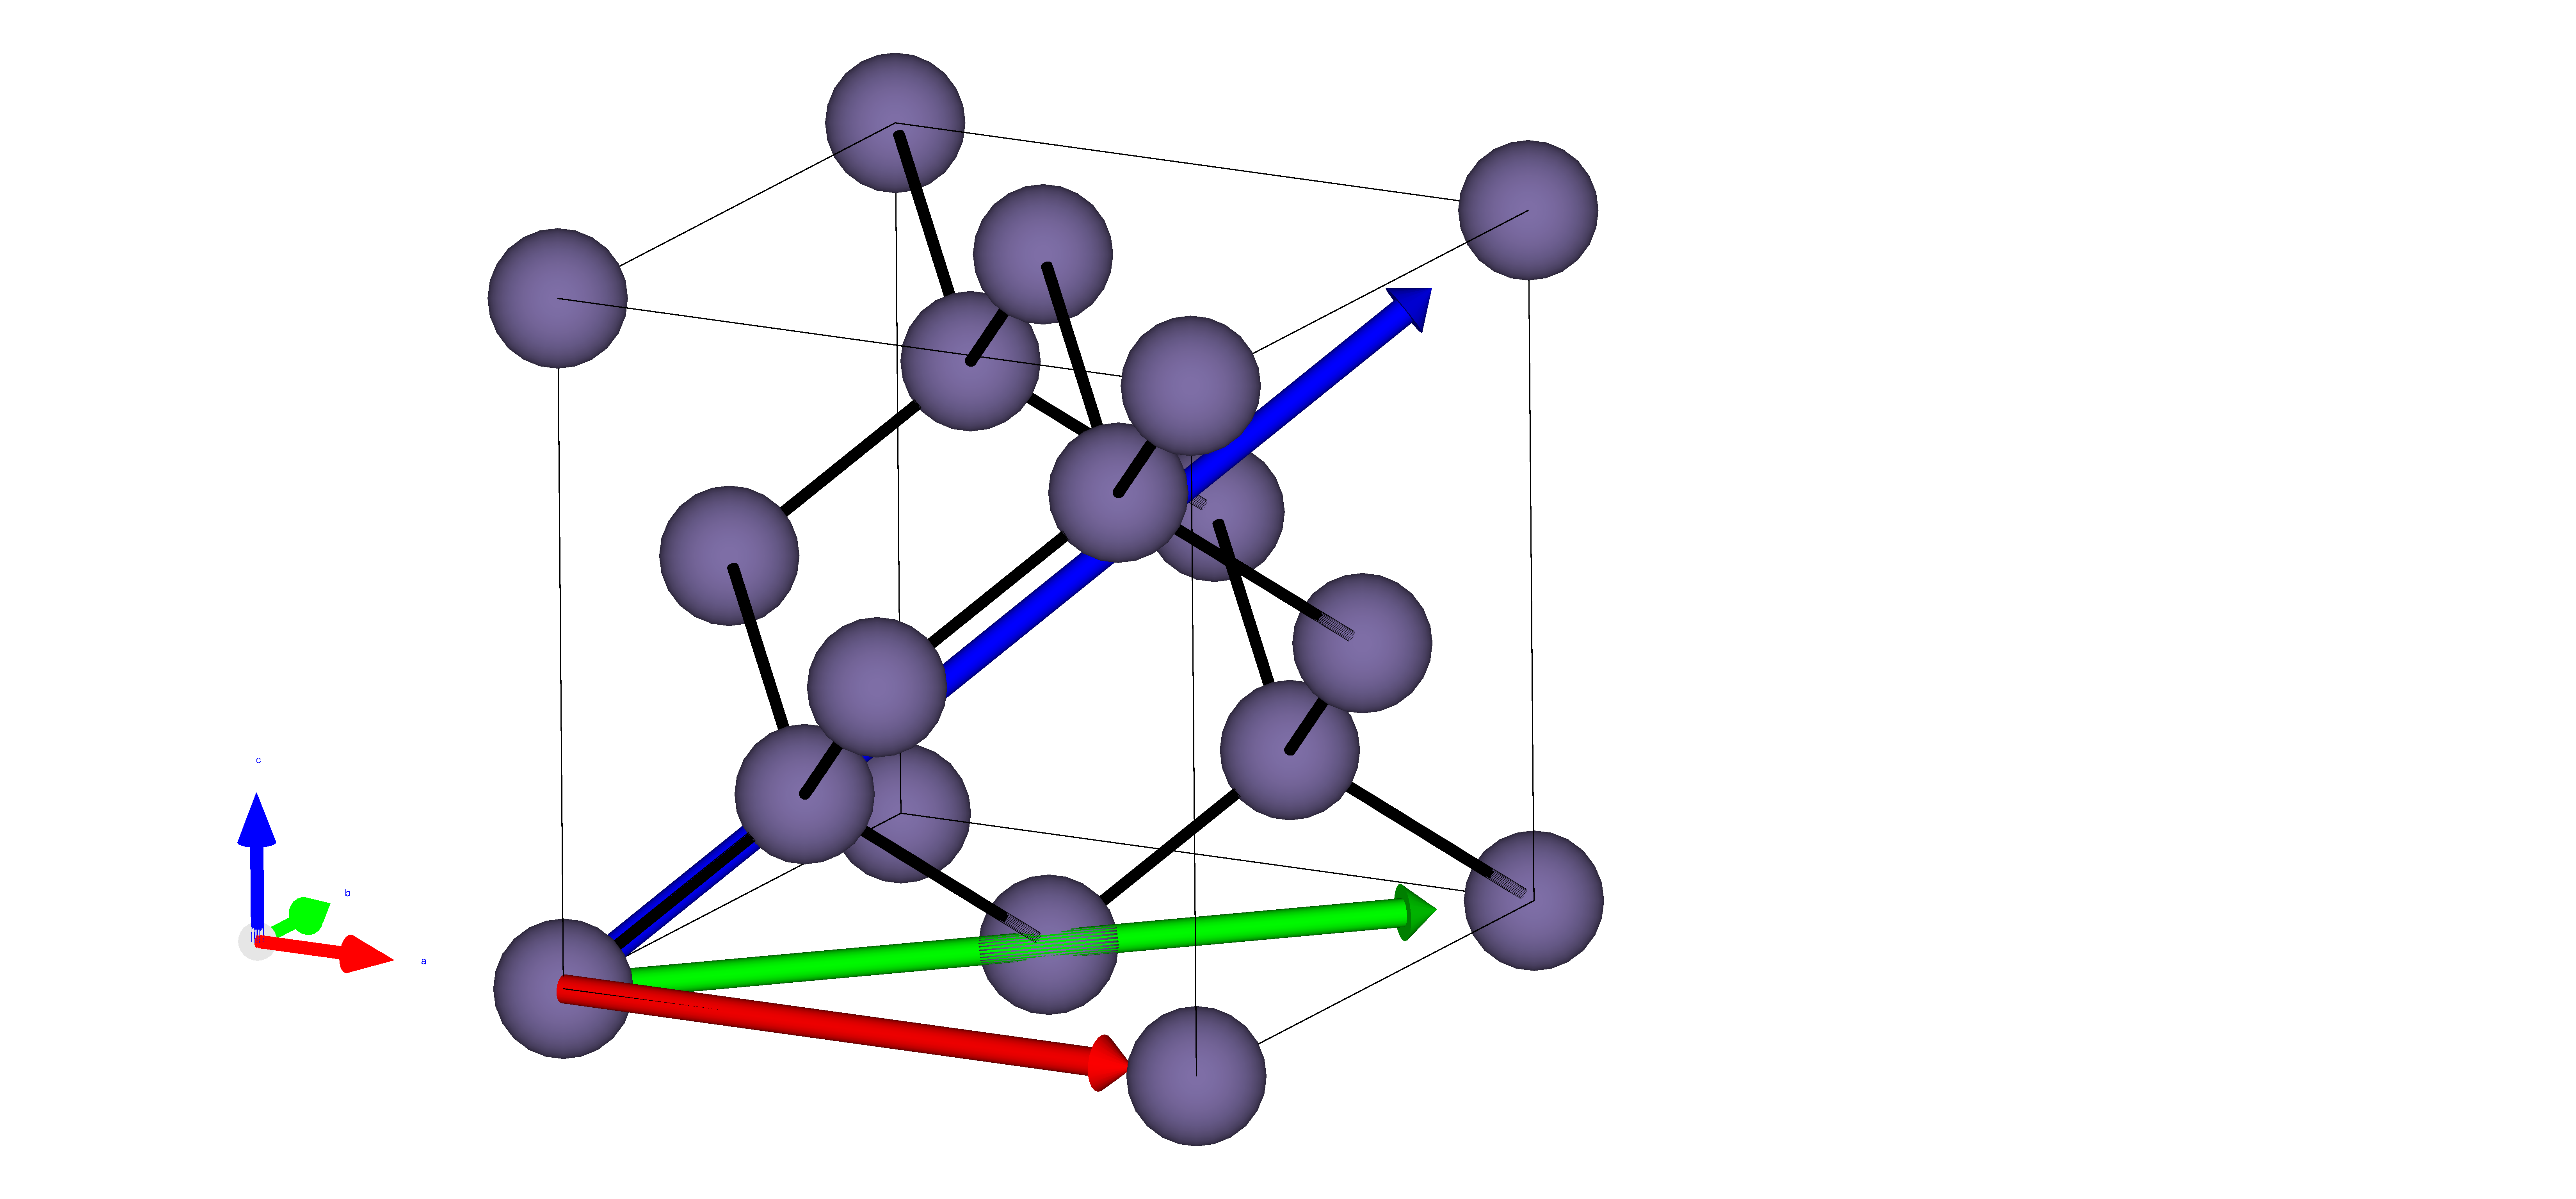
\includegraphics[width=1\textwidth]{strain/strain_direction.pdf}
	\caption{Relevant strain directions in diamond structure: \textcolor{red}{$[100]$}, \textcolor{green}{$[110]$}, \textcolor{blue}{$[111]$}.}
	\label{Fig:strain_direction}
\end{figure}

After defining strain types, the range of staining must be set as well. In the literature, many articles can be found, both experimental and theoretical, concerning strains and their effects on electronic properties \cite{strain-limit1,strain-limit2,strain-limit3}.
Both compressive and tensile strains are investigated, usually in the range of maximum $4\sim5\%$ of equilibrium lattice constants.
Due to practical issues and technological limitations, the range of research conducted is up to $4\%$.
From now on, there will be used such a convention that: the tensile strains will be represented by positive numbers, while compressive ones with negative.
Although of main interest was the effect of strain on electronic structure the investigation began with studying the structural properties, i.e. the effect of axial and biaxial strain on lattice parameters and atomic positions.

At first, for every system, the lattice represented by \prim\ were optimized and equilibrium lattice parameter were established.
Then the negative and positive isotropic strain was applied by elongating/shortening the lattice parameter, and respective stress (pressure in this case) was found.
In the next step, the response to biaxial and axial strain with respect to directions $[100]$, $[110]$ and $[111]$ was evaluated.
The optimization algorithm has difficulties with atomic positions improvement in \prim, due to lack of atoms to interact with.
For that purpose the appropriate supercells were constructed, strains were applied, the remaining structural degrees of freedom (the lattice and atomic ones) were optimized, and the induced stress was evaluated.

Supercells are a stack of crystallographic cells, in certain or multiple directions, that are built usually to optimize atomic structure, create alloys and admixtures (periodic boundary conditions), or add defects to structure, or simulate surface effects.
Those made for diamond structure calculations are shown on figure \ref{Fig:supercells}.

\begin{figure}[!htbp]
	\centering
	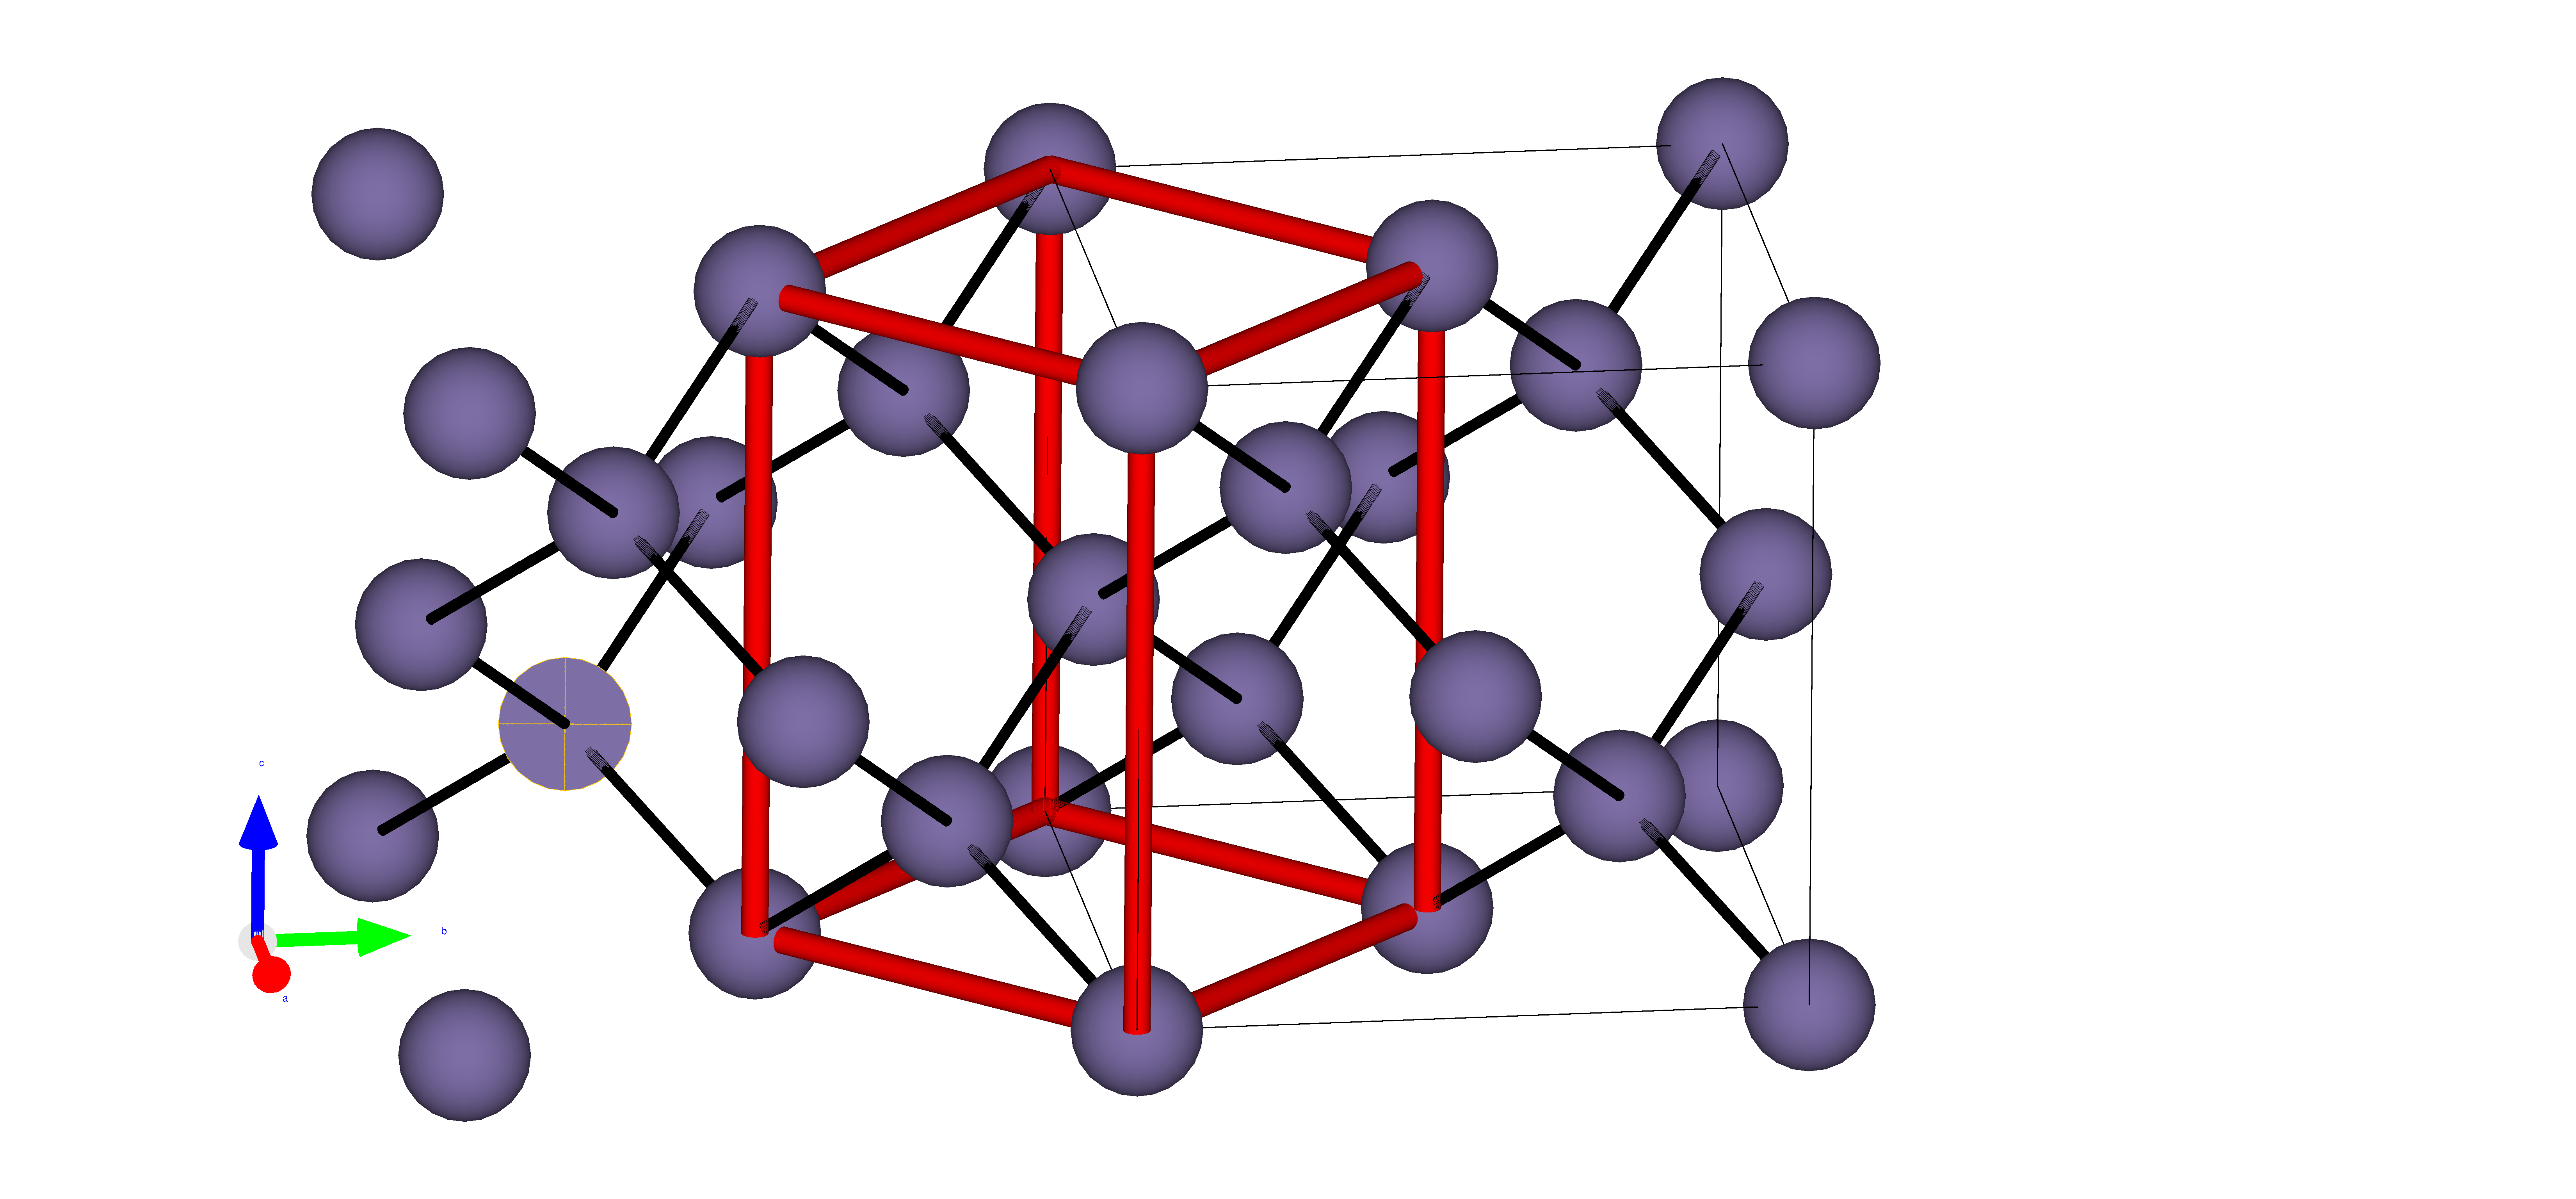
\includegraphics[width=.8\textwidth]{strain/100_supercell.pdf}
	\caption{Supercell for optimization in [100] and [110] strain directions.}
	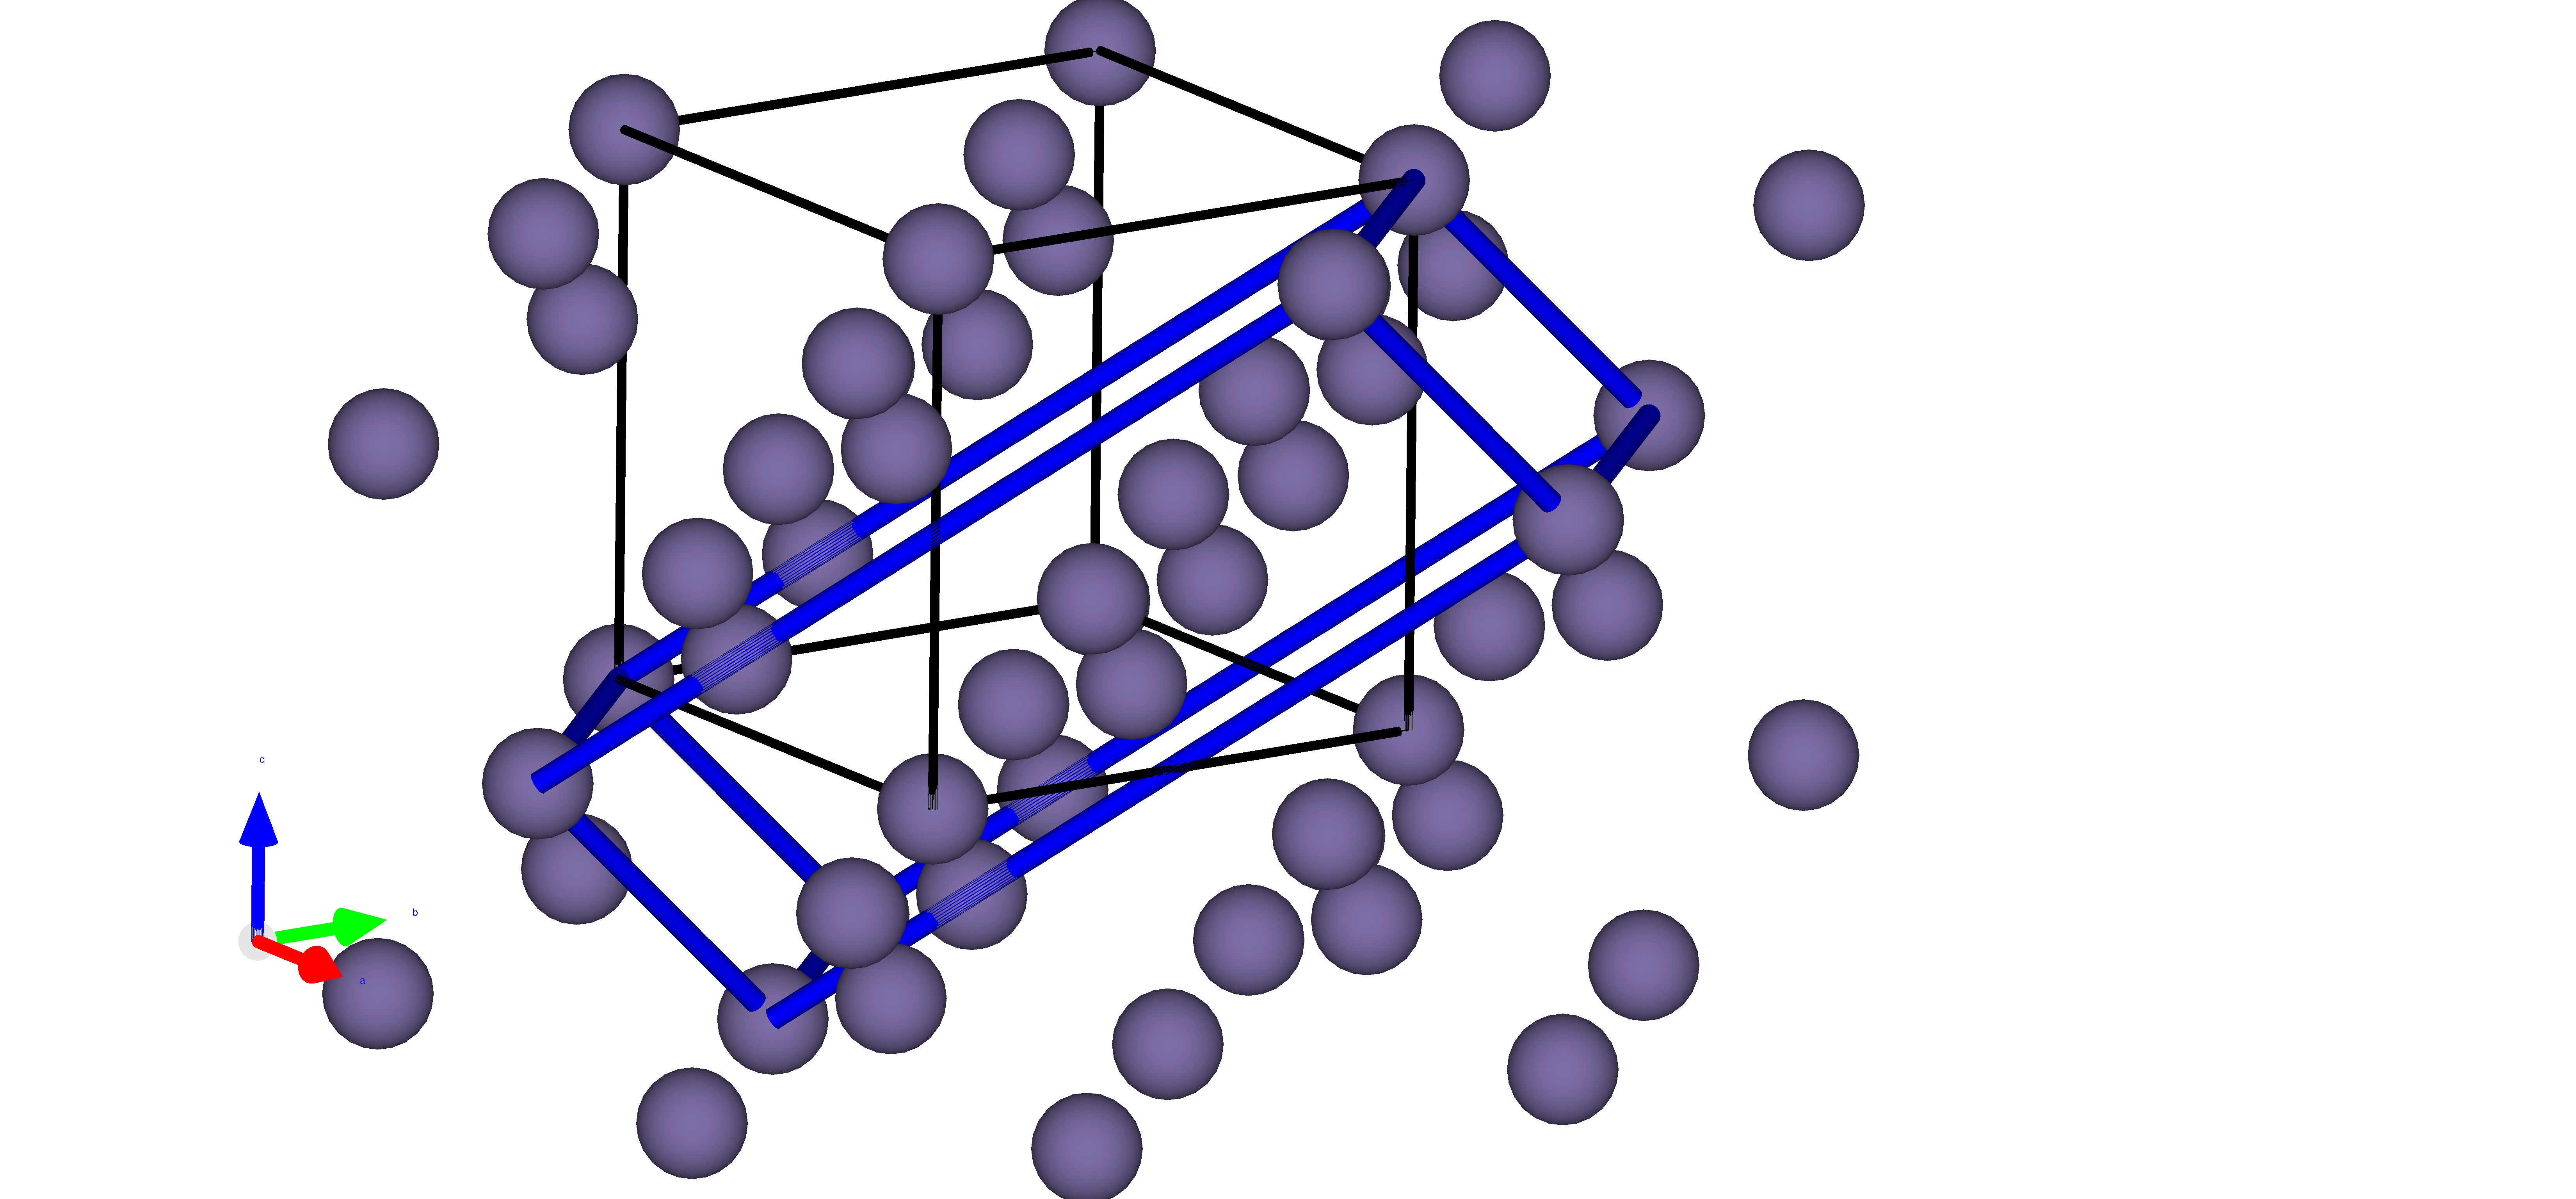
\includegraphics[width=.8\textwidth]{strain/111_supercell.pdf}
	\caption{Supercell for optimization in [111] strain direction.}
	\label{Fig:supercells}
\end{figure}

While constructing supercell it is crucial to remember what direction of strains will be applied.
In case of ABINIT package, during non--isotropic relaxation of cell shape, at least one lattice vector must be orthogonal to the remaining two.
Moreover, crystallographic directions, in which strain must be induced, must lay along lattice vectors.
Only then chosen direction dimension may be fixed.
Obviously, in case of planar strains, there is no need for that, as long as plane of strains is parallel to a plane spread on two of the lattice vectors.
Due to that, and the fact that the diamond structure has cubic symmetry, it was possible to construct one supercell for both $[100]$ and $[110]$ directions of strain.
Unit cell for $[111]$ direction was not obvious to construct.
One lattice vector must follow diagonal of the conventional cell.
As for the rest, nearest neighbours to $(0,0,0)$ atom in perpendicular plane to diagonal had to be found.
This led to hexagonal symmetry cell, of $120^\circ$ between non--diagonal lattice vectors.

Supercells constructed for applying strain in $[100$ and $[110]$ directions, and it's lattice vectors $a_1'$, $a_2'$ and $a_3'$, can be described by transformation matrix from conventional cell as

\begin{equation}
\label{Eq:trans_100}
\begin{bmatrix}
a_1' \\ a_2' \\ a_3'
\end{bmatrix}=
\begin{bmatrix}
0.5 & 0.5 & 0 \\
-0.5 & 0.5 & 0 \\
0 & 0 & 1
\end{bmatrix}
\begin{bmatrix}
a_1 \\ a_2 \\ a_3
\end{bmatrix},
\end{equation}

while for [111] as

\begin{equation}
\label{Eq:trans_111}
\begin{bmatrix}
a_1' \\ a_2' \\ a_3'
\end{bmatrix}=
\begin{bmatrix}
0.5 & 0 & 0.5 \\
-0.5 & -0.5 & 0 \\
-1 & 1 & 1
\end{bmatrix}
\begin{bmatrix}
a_1 \\ a_2 \\ a_3
\end{bmatrix}.
\end{equation}

All strains were applied in the range between $-4\%$ and $4\%$ of frozen respective lattice parameters and the structures were optimized without symmetries imposed (except identity) to avoid symmetry induced fixing of atomic positions.
To characterize the structural changes, the Poisson's ratio was used, defined both for the axial and biaxial strains as:

\begin{equation}
\label{Eq:poisson}
\poisson=-\frac{\epsopt}{\epsind},
\end{equation}

where $\epsind$, $\epsopt$ are respectively induced and optimized relative changes in a linear dimension along the considered direction and in the plane perpendicular to it. It should be mentioned that the isotropic behavior of a system around chosen axis takes place only for $[100]$ and $[111]$ directions.
For $[110]$ the Poisson's ratio defined above is not a well established quantity since under axial strain the relative expansion/contraction is not uniform around the axis and is the highest for $[001]$  and the lowest for $[1\bar{1}0]$.
Similarly, a uniform strain around $[110]$ axis leads to non-uniform stress.
Nevertheless, the $[110]$ direction has also been considered, with plane degrees of freedom naturally optimized under axial strain and biaxial strain applied uniformly, which may take place if a substrate in epitaxial technology is $(110)$ surface of a cubic symmetry crystal.
It is worth mentioning here that, from the definition, Poisson's ratio is defined for uniaxial strain, and falls within the range of $0-0.5$.
To be able to compare results from uniaxial and biaxial strain types, pseudo--Poisson's ratios ware also calculated for biaxially strained systems (later also called Poisson's ratio).

The resulting stresses ($\stress$) appearing at induced strains are described by respective elastic constants, first ($C1$) and second order ($C2$), so that the stress is given by the formula:

\begin{equation}
\label{Eq:stress}
\sigma=\text{C1}\cdot \epsind+\text{C2}\cdot \epsind^2.
\end{equation}

In the above formula $\epsind$ is a fractional relative change of a given dimension and the constants $C1$ and $C2$ are expressed in $GPa$. For the case of $[110]$ uniform biaxial strain there are two values of $C1$ and $C2$, corresponding to $[001]$ and $[1\bar{1}0]$ directions.
It should be noted that the elastic constants defined above are not directly related to standard elastic matrix elements.
However, for verification purposes the standard elastic constants have been derived from presented results and compared with the textbook data.
In the case of cubic symmetry there are only three non-zero and independent elastic constants ($c_{11}$, $c_{12}$, $c_{44}$).
All of them have been calculated from $C1$ and $C2$ values via standard transformation rules of stress tensor.
\footnote{Derivation of elastic constants from obtained results can be found in appendix \ref{chap:derivations_stress}}
Because of small differences in results for different strain directions, the average values and standard deviations are given in part \hyperref[part:III]{\Romanbar{III}}.

In the next step, the electronic structure was studied.
Supercells are inconvenient for band structure analysis, due to their sizes which, on the other hand, change volume or even shape of \BZ.
That makes it difficult to find meaningful points in \BZ\ and moreover causes problems with folding of bands.
To avoid the problems in supercells mentioned before, they have been transformed back to \prim.
The detailed derivation of transformation is described in appendix \ref{chap:derivations_supercell}.
Owing to such an approach the changes in the electronic band structure could have been easily followed since the relative positions of characteristic points in the deformed by strain \BZ\ remained unchanged with respect to the equilibrium state \BZ.
Of the main focus were characteristic energy gaps between \VB\ and \CB, $\Gamma$--$\Gamma$ (direct band gap), $\Gamma$ -- minimum along $\Delta$ directions and $\Gamma$ -- minimum along $\Lambda$.
The expected splitting of energies within $\Delta$ and  $\Lambda$ stars caused by symmetry breaking can be observed.
In the case of strained systems, where there is a lack of experimental data, the \textit{c} parameter (Eq. 3 in \cite{mBJLDA}) (responsible for the band gap value) was set as follows
\begin{equation}
\text{c}^{st}=\text{c}^{st}_{sc}\cdot\frac{\text{c}^{eq}_{fit}}{\text{c}^{eq}_{sc}},
\label{Eq:ctbo9}
\end{equation}
where \textit{st} means strained, \textit{eq} -- equilibrium, \textit{fit} -- fit to experiment, \textit{sc} -- \SC\ value.

At this point also the effective masses have been evaluated as functions of strains.
The calculations of effective masses were performed by fitting the 3rd order polynomial, which was necessary because of asymmetry of the bands around minima.
For the sake of reliability, $5$ to $9$ points around band extrema were taken into consideration, and the densities of points along k-space path were subjected to convergence studies.
In the \CB\ the effective masses at $\Gamma$ point as well as at the valleys along $\Gamma$-$X$ and $\Gamma$-$L$ directions have been calculated, taking into account also the star-degeneracy removal due to the broken symmetry under strain.
In the \VB\ only the top of the band at $\Gamma$ point has been considered, whether it was the heavy or the light hole band (due to inversion of bands).
The effective masses were evaluated from the inversion of the second derivative of fitted polynomial at the extremum.

From quantum mechanics, it is known that, all of the physical observable's changes are smooth.
Which means that non--smooth behaviour must be investigated further.
To better understand non--smoothness appearing in band structure, it is worth to calculate the orbital composition of bands.
In practice it projects band structure on each orbital of every atom in the system allowing to look into symmetry of certain band and trace it's movement along with straining.
Two most common physical effects that usually occur are: band inversion and splitting of bands.
First one happens when bands degenerate, e.g. when band gap closes.
Then former \CB\ moves beneath former \VB.
Second effect may occur during symmetry break.
While breaking the symmetry of the system, usually (depending on actual space group), especially \VB, band might loose it's degeneracy, resulting in splitting.

In the last step, the deformation potentials $a_v$, $a^{dir}$, $a^{ind}$ $b$, $d$, $\Xi_u^{\Delta}$, $\Xi_u^{L}$, as defined in \cite{pot-def} were calculated.
In the calculations of $a_v$, $b$, and $d$, which are absolute in the sense that they describe the changes in absolute positions of some points in bands, the crucial point is to establish the unified energy reference point, i.e. the reference point which do not flow with the strain.
For that purpose we have used the natural slab method \cite{zunger} in which we assume that the energy level in vacuum should not change under strain, and thus defines the energy reference point.
There are also a few rules one should keep in mind preparing the calculations:
\begin{itemize}
    \item for both slab and bulk calculations, it is crucial to set the same k--point grid.
    In a slab a good practice is to adjust number of k--points to slab size.
    E.g. In bulk set k--points to $10\times 10\times 10$, while slab in $[100]$ direction of $5$ layers of material and $5$--layer--long vacuum set to $10\times 10\times 1$.
    That way slab layer and bulk have exactly the same k--points distribution.
    \item vacuum must be long enough for the plateau to be clearly visible.
    the flat area should be wide enough for a small fluctuation to emerge.
    That guarantees the vacuum to clear of slab potential.
\end{itemize}

\begin{figure}
	\centering
	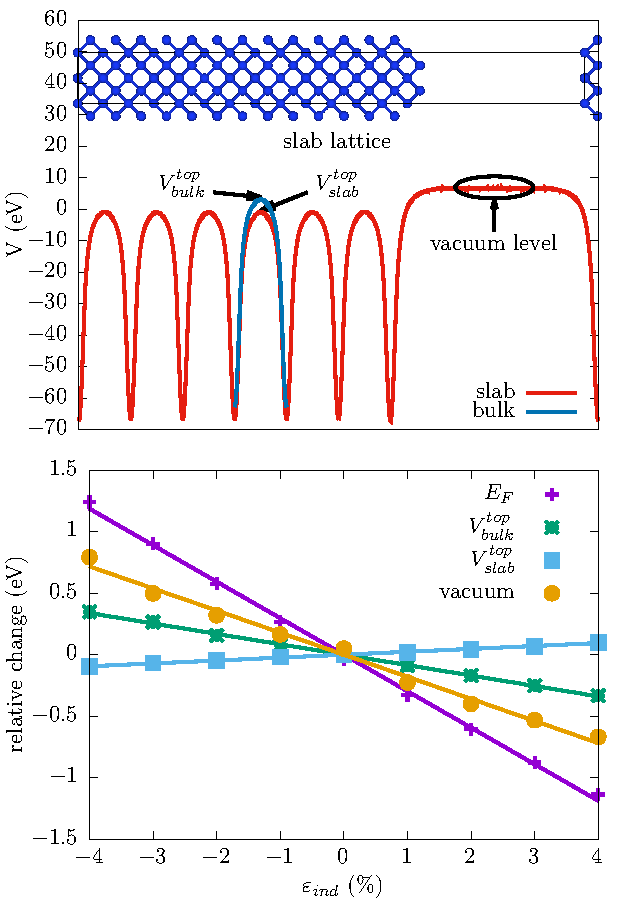
\includegraphics[width=1\textwidth]{strain/offsets.pdf}
	\caption{Illustration to the deformation potential determination procedure, for Si under isotropic strain. Upper figure: the lattice used and the \SC\ potential throughout this lattice (red line) as well as corresponding potential in bulk (blue line). Lower graph, the strain induced energy variations necessary to evaluate the deformation potential.}
	\label{Fig:offsets}
\end{figure}

Figure \ref{Fig:offsets} illustrates where the partial data are taken from in the calculations of $a_v$ in Si under isotropic strain.
To establish the unified energy reference point we apply the following assumptions: i) the vacuum level should not change under strain, ii) The rates of the changes in the \SC\ potentials at chosen point in bulk and equivalent point in the slab, under strain, should be the same.
Thus, when defining the linear coefficient of lines in Fig. \ref{Fig:offsets}: $a^F$ - \VBM, $a^{Vb}$ - \SC\ potential value at chosen point in bulk (maximum), $a^{Vb}$ - \SC\ potential potential value at equivalent point in the slab, $a^{Evac}$ - energy level in vacuum, the deformation potential $a_v$ can be calculated from the formula:

\begin{equation}
\label{Eq:av}
a_v=(a^F - a^{Vb} + a^{Vs} - a^{Evac})\cdot100/3,
\end{equation}

where the factor $100/3$ comes from the transformation from percent to fraction, and from linear to volume change.

The corresponding uncertainties have been calculated from linear coefficients uncertainties in \abinitio\ data approximations, assuming the ''worst case'': 

\begin{equation}
\label{Eq:Dav}
\Delta(a_v)=[\Delta(a^F) + \Delta(a^{Vb}) + \Delta(a^{Vs}) + \Delta(a^{Evac})]\cdot100/3.
\end{equation}

The described procedure was used in the calculations of all the absolute deformation potentials.
In the calculation of relative deformation potentials $a^{dir}$, $\Xi_u^{\Delta}$, $\Xi_u^{L}$ the procedure is not necessary because when calculating the energy differences (e.g. $E_c-E_v$) the subtracted energies are always given with respect to the same energy reference point.

Thus, in the calculations the same supercell as for the $[100]$ and $[110]$ structure optimizations have been used except a vacuum layer has been added, i.e.  $3-4$ layers of optimized supercell and $6-7$ supercell--layers--long distance of vacuum.
The total potential across the whole supercell (in the direction perpendicular to the slab) was evaluated for slabs with and without separating vacuum layer.
As a result the energy variation slopes described above were found, corresponding to respective deformation potentials.

\ornament

\section{Alloying}
\label{sect:alloy_theory}

In this part of work all calculations were performed with ABINIT software package.

Second presented method of band structure engineering is alloying.
Creating alloys and admixtures of different materials (even slightly) can drastically change materials properties, especially in case of semiconductors, which are known for their huge sensitivity for impurities.
Main difference between alloying and doping is percentage of admixture.
It is worth noting that low (light) doping is considered to be, when one dopant atom is added per 100 million atoms, while heavy (high) doping per ten thousand atoms.
Alloy, on the other hand, is concerned when admixture is per one hundred atoms and less.

In case of silicon technology impurities are usually added in bulk growth process.
Proper application of this technique provides nearly uniform impurities doping in each silicon wafer.
Also through photolithography, the process of doping selected areas can be conducted by diffusion and ion implantation (high control over the process).

Before getting further into band structure engineering it should be stated what within this thesis 'alloy' actually means.
The concept of alloy is quite vast and covers many different material types.
From uniform materials to multi--phase ones, including all types of doping in atomic scale.
A doping atom can substitute base atom, create vacancy or fit in interatomic position.
That gives large field of study, too big actually to cover all this cases in research.
Thus some choice has been made.
In this work only uniform phase with substituting base atom is taken under consideration.

The active region of modern optoelectronic devices (detectors, light emitting diodes, lasers, etc.) is often based on semiconductor alloys.
They offer an opportunity of tuning the band gap by varying their composition.
One of materials of interest in the field is the $\mathrm{Ge_{1-x}Sn_x}$ alloy \cite{homewood15, shigeaki15, margetis17, jeremie19, tran19}.
Its direct gap can be tuned in the range of $0.89-0$ eV by varying the composition \cite{growth,sigesn, Polak_2017, zhao20}.
Additionally, it exhibits an interesting property, where by varying the alloy composition, a transition from indirect to direct band gap is possible.
This transition appears at a relatively small admixture of Sn in Ge (around $6.5\%$) (e.g. \cite{Polak_2017}).
This feature, joined with the observed high mobility of carriers, makes this material a promising candidate for optoelectronic applications.
This fact has been a reason for an extensive experimental and theoretical investigations of this material, e.g. \cite{sigesn, Polak_2017, snge, zhao20,growth,PhysRevLett.79.1937,gesn-engineering,vegard,sisnge,gesn-0.14,ge_alloy_compare,electroreflectance, random_alloys,doi:10.1063/1.125558,SAHNOUN2005392,Moontragoon_2007,PhysRevB.78.161203,small_sn,ZHANG201212,article,doi:10.1063/1.4790362,HUANG201443,PhysRevB.89.165201,coherent_approx,C5CP02558C}.
In particular a number of \DFT\ based \abinitio\ theoretical studies have been conducted \cite{Polak_2017, zhao20, snge, random_alloys,doi:10.1063/1.125558,SAHNOUN2005392,Moontragoon_2007,PhysRevB.78.161203,small_sn,ZHANG201212,article,doi:10.1063/1.4790362,HUANG201443,PhysRevB.89.165201,coherent_approx,C5CP02558C}.
It is a known fact that the \abinitio\ methods provide very realistic predictions of properties of atomic systems but often at a high computational costs.
In the case of alloys, the method of choice is the use of periodically repeated supercells containing up to a few hundred of randomly distributed atoms of species forming the system, which makes the calculations computationally time consuming \cite{PhysRevB.89.165201,coherent_approx,C5CP02558C,Polak_2017}.
The most prominent advantage of this method is the ability to include lattice distortion around impurities, as well as vacancies in the structure and even interatomic position dopants.
Although, in such approach only a discrete number of compositions can be analyzed.
Also, the problem emerges in choice of atoms substituted in whole supercell, such that it would statistically represent the best bulk material.
For that purpose \SQS\ (Special Qausirandom Structures) \cite{sqs} are usually used.
Although, it should be kept in mind that they only increase the chance to statistically well represent the material.
More important is appropriate size of supercell.
Moreover, the use of large supercells results in numerous folded bands which makes the interpretation of the picture of the band structure rather complicated.
The necessary unfolding procedure \cite{unfolding} provides an effective band structure represented in the form of spectrally weighted eigenvalues, which are the more torn and blurred the more percentage of admixture.
That makes their direct application in modeling of semiconductor devices very inconvenient, due to often large blur of bands.
For this reason, in device modeling other representations of electronic bands are most often used, among which the $\mathbf{k}\cdot\mathbf{p}$ method seems to be the most popular \cite{richard05, kurdi10, gladysiewicz13, gladysiewicz14, maczko19}.
These methods require certain number of parameters which are found from fitting either to experimental data or to large scale \abinitio\ calculations.

For this task is applied an approach which joins large scale \abinitio\ calculations with 30-band $\mathbf{k}\cdot\mathbf{p}$ method, which is known to correctly reproduce the electronic band structure in the full \BZ.
This approach allows to find the values of the parameters used in the $\mathbf{k}\cdot\mathbf{p}$ method.
Finding them directly from \abinitio\ supercell data would be difficult (if possible at all), due to the character of the obtained band structures.
Therefore, it is proposed to make an intermediate step which is based on other \abinitio\ approaches.

Despite supercell method there are basically three more methods suitable for alloy calculations.
First one, and the simplest, is Virtual Crystal Approximation \cite{vca1} (\VCA).
In practice, each site occupied by more than one different atom type is set with virtual atom interpolating behaviour of site components.
By that, it ignores all short range interactions around disordered site, what follows possible local lattice distortion.
The advantage of this method is low computational cost, of the order of ordered structures.
Either way, \VCA\ was useful enough to be modified in various manners, suitable for specific group of materials \cite{vca_mod1,vca_mod2}.
Second approach is so--called Coherent Potential Approximation (\CPA).
It is physically the most sophisticated method, as it is supposed to model scattering properties of disordered system.
This approach is appropriate for Green's function formalism, in which \KKR\ method is implemented.
Unlike \VCA, the \CPA\ instead of mixing potentials and creating average atom, it mixes Green's function of whole system with all of the components separately.
Moreover in different combinations (if the site has more equivalent positions).
That way, it  approximates a configurationally random alloy with an effective medium that is determined self-consistently from the condition of stationary scattering.
On the other hand, it is insufficient for geometry optimisation or total energy calculations.
Due to that, impurities which highly distort lattice will not be well represented.
Third method available is Computational Alchemy.
This one bases on perturbation theory to calculate the response to the difference of \VCA\ potential and the real one.
One can treat this approach simply as a correction to \VCA.

Because \CPA\ method requires Green's function approach and as output gives Bloch's spectral function instead of typical band structure, that method also was rejected for device modeling purpose.
\VCA\ on the other hand is not accurate enough method due to its simplicity.
Thus a computational alchemy was chosen, as a more reliable technique than \VCA\ and applicable unlike \CPA\ and supercell calculations.

The approach has already been exploited in a number of works, e.g. \cite{ingap_alch,gesi_mc_alch,alloys_alch,vca}.
The ABINIT package was used with implementation of the computational alchemy, called the Alchemical Mixing (\AM).
The \AM\ itself is known to provide rather poor description of electronic structure, particularly for highly mismatched alloys (\HMA), mainly because it does not account for the local distortions of the lattice \cite{ingan}.
However, when used as a model containing additional fitting parameters it is able to accurately reproduce the band structure for any composition of an alloy at low computational costs.
Thus, at the first step, the \AM\ method is used to approximate the reference supercell unfolded band structures.
Next, the continuous \AM\ bands are used to find the values of the parameters of 30-band $\mathbf{k}\cdot\mathbf{p}$ model, through a specially designed optimization method.
As a result, an effective full \BZ\ electronic band structure description of the $\mathrm{Ge_{1-x}Sn_x}$ alloy in the full composition range is obtained.

As mentioned above, to approximate the \abinitio\ supercell band structure we the concept of computational alchemy has been used, as implemented in the ABINIT code \cite{abinit1} and called the alchemical mixing (\AM) there.
The idea is similar to the \VCA\ \cite{vca}, often used to describe mixed crystals within empirical potential approach.
In the \AM\ approach a scattering center (ion) is created whose properties reflect the properties of two ions simultaneously, at a given proportion.
The \VCA\ relies simply on a linear combination of two one-electron potentials of parent compounds.
The alchemical mixing of pseudopotentials implemented in the ABINIT package uses the following construction \cite{abinit2}:
\begin{itemize}
    \item the local potentials are mixed in the proportion given by mixing coefficients,
    \item the form factors of the non-local projectors are all preserved,
    \item the scalar coefficients of the non-local projectors are multiplied by the proportion of the corresponding type of atom,
    \item the characteristic radius of the core charge is a linear combination of the characteristic radii of the core charges,
    \item the core charge function $f(r/rc)$ is a linear combination of the core charge functions.
\end{itemize}

In all the linear combinations the mixing coefficients reflect the proportion at which particular atoms enter the alloy are used.
In the approach only the atoms with the same valence electronic configuration can be taken (isovalent elements, like e.g. Ge and Sn).
In this work the Hartwigsen-Goedecker-Hutter (\HGH) pseudopotentials \cite{hgh} have been used.

There is a lot of freedom in choosing the mixing proportions, the only constrains are that the overall formula $\mathrm{Ge_{1-x}Sn_x}$ must be fulfilled at every composition, and that the content of an element in an \emph{alchemical} atom must not be negative.
There has been used a scheme which, on the one hand, guarantees a consistency of mixing for any composition and, on the other hand, allows, in some extent, to check the effect of mixing proportions on the results.
The two \emph{alchemical} atoms representing two sublattices in \BZ\ structure, $A1$ and $A2$, are composed from Ge and Sn atoms according to the formulas:

\begin{align}
\label{Eq:mixing}
\begin{split}
A1=Ge[(1-x)+\alpha x(1-x)] + Sn[(x)-\alpha x(1-x)]\\
A2=Ge[(1-x)-\alpha x(1-x)] + Sn[(x)+\alpha x(1-x)]
\end{split}
\end{align}
where $\alpha$ is a parameter responsible for the proportion of mixing and can be varied in the range $[0,1]$.
The mixing parameter $\alpha$, if non--zero, allows to add a bowing to the mixing curve versus the amount of admixture, and what follows, to not equally occupy chosen site by component atoms.
Testing it's impact on results is vary important.
Value of $\alpha$ resembles the arrangement of atoms in supercell.
What follows, in larger cells with higher number of independent sites, the obtained results can be sensitive to the choice of mixing parameter.

One of the advantages of the \AM\ approach is a significant reduction of system size to be analyzed from first principles, which can be reduced to a \prim.
However, the accuracy of such approach is questionable, in particular it does not account for the local distortions of the lattice \cite{ingan}, which is significant in \HMA s where the local relaxation effects play a crucial role \cite{Polak_2015}.
Nevertheless, the \AM\ approximation, when used together with supercell calculations \cite{Polak_2017} as reference, can be very useful.
When properly adjusted to the supercell data, they may provide a very good approximation of electronic bands with continuous curves.
Therefore, there was designed a procedure of utilizing the \AM\ approach in a way that allows to reproduce results obtained with more accurate methods, including supercell \DFT\ calculations and experimental measurements.
In this chapter is demonstrated the applicability of the method with results of \DFT\ supercell calculations serving as reference.

There are only two key parameters necessary to achieve realistic band gaps:
\begin{enumerate}
    \item lattice constant,
    \item $c$ parameter from \mBJLDA.
\end{enumerate}

Each provides different changes to band structure and must be considered with respect to the other one.
Usually, in case of semiconductors, direct and indirect band gaps are to be well modeled.
As it is shown in \ref{chap:strains}, manipulating lattice constant (compressing or stretching material isotropically) closes or opens band gaps.
Major visible effect is shift of whole bands.
Although it should be pointed out that changes between certain valleys on the same band will appear.
And for that second reason lattice constant is used.

On the other hand $c$ parameter in functional serves to manipulate distance between valence bands and conduction bands (which is the purpose of \mBJLDA\ functional).
Also this parameter changes ratio between direct and indirect band gap, due to bands flattening.
The effect is not strong but must be taken into consideration while increasing fitting accuracy.

As first lattice constants should be evaluated.
Due to fitting nature of this method, at the beginning must be found such constants that would give proper band gaps on boundary conditions.
In the case of $\mathrm{Ge}_x\mathrm{Sn}_{1-x}$ band gaps and and other necessary parameters (like $c$ parameter in \mBJLDA\ \ref{Eq:c_mbj}) can be taken from strain calculations.

After obtaining lattice constants with correct band gaps it is necessary to be able to achieve accurate constants for any alloy composition.
Usually for that purpose Vegard's law is applied \cite{vegard1}.
It states that the lattice constant for chosen alloy composition is linear combination of lattice constants of alloy composing materials equivalent to percentage of mixing.
It should be noted that there are many exceptions from Vegard's law \cite{vegard2,vegard3,vegard4}.
Such an exception is $\mathrm{Ge}_x\mathrm{Sn}_{1-x}$ as well \cite{Polak_2017}.
In lattice constant vs composition occurs visible bowing.
Due to that fact, to properly model the whole range of composition, another point on the curve or bowing parameter is necessary to duplicate supercell results.

While $\mathrm{Ge}_x\mathrm{Sn}_{1-x}$ does not obey Vegard's law, other materials usually obeying stated relation might still need to include a bowing.
The main goal is to accurately describe band gaps characteristics.
If material obeys Vegard's law but the \AM\ band gaps are inaccurate with real lattice parameters, there might be a need to manipulate lattice constant to achieve an agreement with experimental / supercell results.

What is left is a choice of searching algorithm.
There are only two parameters.
The easiest way (and maybe the most efficient one) is work on bowing parameters for lattice constant and $c$, instead of actual values.
That way, there is only a need to specify two variables to generate whole stack of calculations for each admixture amount, that experimental (or supercell) data are provided.

Having parameterized necessary variables, band structure calculations can be performed.
The procedure for that calculations, as well as estimating effective masses of charge carriers, is equal to strain research that was described previously (\ref{sect:alloy_theory}).

\ornament

\section{Structural factor}

In this part of work all calculations were conducted with VASP software package.

The third method of electronic structure engineering, mentioned in the introduction, is the formation of alternative (metastable) crystal structures.
Modern deposition technologies, like molecular beam epitaxy (MBE) or metal--organic chemical vapor deposition (MOCVD), open such opportunities.
Usually the structure is induced by the substrate (e.g. wurtzite structure by the (111) surface of zinc blende crystal).
In principle any crystal structure can be formed, but the most important issue is the stability and thermodynamic stability of the system.
It is a known fact that the diamond structure is the stable one for Si and Ge, however, for C itself (diamond) is a metastable structure, and although rather difficult to be formed it is a well known system and has various applications, in jewelery in particular,  but not only.
Diamond owing to its exceptional hardness, very high thermal conductivity (phonon induced), very good electrical insulation properties, transparency for light, has various applications in technics, e.g. diamond anvil cells for creating the high pressure environment.
This example shows, that the formation of metastable crystal structures is an open way in the band structure engineering.

In this work only the wurtzite structure will be taken into consideration, since it is energetically very close to the diamond one, and relatively easy to obtain, by deposition on the (111) zinc blende plane.
Some properties of such structures of Si and Ge are already known \cite{wz_si_exp1,wz_si_exp2,wz_si_exp3,wz_si_exp4,wz_si_exp5,wz_ge_exp6}, in particular it turns out that the fundamental band gap in Ge is direct, (unlike in the diamond structure) which is a crucial feature in optoelectronics.
It is worth mentioning that mostly Si was investigated, while Ge barely exists in the literature.
The available data range from achievement of Si wurtzite nanowires \cite{wz_si_exp1}, \abinitio\ studies of strained Si, through vibrational \cite{wz_si_exp2} and doping properties \cite{wz_si_exp3,wz_si_exp4}, up to Raman spectrum of Si \cite{wz_si_exp5}.
Apart from the formation energies, the elastic constants and the Poisson ratio, the systematic investigations of the effect of strains has been performed, for C, Si and Ge.
The isotropic (pressure), biaxial (perpendicular to c--axis) and axial (along c--axis) strains have been considered.
In particular the effect of strains on the band structure and its crucial features: band gaps (identification of fundamental gaps) and effective masses.
Such calculations have allowed also to evaluate the deformation potentials, crucial parameters in the calculations of superstructures electronic bands and of the electron--phonon coupling. 


For all of the calculations presented here, VASP \cite{vasp1,vasp2} software package was used, mainly due to implementation of \mBJLDA\ on \PAW\ pseudopotential.
The procedure was similar to the one presented in Chpt. \ref{chap:strains}.
Although, there are a few differences in methodology:
\begin{enumerate}
	\item The anisotropic strains are considered only with respect to one, [001] axis, which is typical when the structure is grown on (111) ZB substrate. The wurtzite cell is presented in Fig. \ref{Fig:wz_cell}.
	
	\begin{figure}[!htbp]
		\centering
		\includegraphics[width=0.7\textwidth]{/wurtzite/wz_cell2.pdf}
		\caption{Conventional cell of wurtzite (\#186).}
		\label{Fig:wz_cell}
	\end{figure}
	
	\item The conventional cell reflects the symmetry of the system, and its possible breaking in the case of anisotropic strains. In wurtzite structure the [001] strains do not lower the symmetry of the cell. What follows the \BZ\ stays the same, and no additional points must be observed. The \BZ\ of wurtzite is shown in Fig. \ref{Fig:wz_BZ}.
	
	\begin{figure}[!htbp]
		\centering
		\includegraphics[width=.6\textwidth]{/wurtzite/186.pdf}
		\caption{First Brillouin Zone of wurtzite crystal structure (\#186).}
		\label{Fig:wz_BZ}
	\end{figure}
	
	\item The differences in the formation energies between WZ and ZB structures is evaluated, to show the energetic preference. This also  gives some hints about stability, especially while straining the system. The thermodynamic stability remains still an open question which require  an independent investigations (lattice dynamics).
	
	\item In wurtzite materials two additional values seem to play important role as $\mathbf{k}\cdot\mathbf{p}$ parameters: the $\Delta_{so}$ and $\Delta_{cr}$. They are connected to \SO\ coupling and crystal field, and are known to be present in wurtzite crystals, and calculated as follows \cite{birpikus}:
	\begin{align}
		\Delta_{so} &= \frac{\Delta_1+\Delta_2}{2} - \frac{1}{2} \frac{c}{a^2}\cdot \sqrt{\Delta}  \\
		\Delta_{cr} &= \frac{\Delta_1+\Delta_2}{2} + \frac{1}{2} \frac{c}{a^2}\cdot \sqrt{\Delta}
	\end{align}
	where
	\begin{align}
		\Delta_1 &= \HH-\LH  \\
		\Delta_2 &= \HH-\CH  \\
		\Delta = \bigg(\frac{c}{a^2}\bigg)^{-2}\cdot (\Delta_1+\Delta_2&)^2-4\cdot\frac{a^2}{c}\big((\Delta_1+\Delta_2)^2-(\Delta_1-\Delta_2)^2\big)
	\end{align}
	
	\item Because of different symmetry compared to the diamond one the deformation potentials also differ as well as the way of calculating them. For wurtzite systems (including \SO) band structure deformation potential ($D_1$ to $D_6$) are defined by the equations \cite{birpikus}:
	\begin{align}
		\Delta E_1 &= E_1 - E_1^0 = (D_1 + D_3)\varepsilon_{zz} + (D_2 + D_4)(\varepsilon_{xx} + \varepsilon_{yy}) +\notag\\ &+\frac{D_6(E_1^0-E_2^0-E_3^0)(\varepsilon_{xz}^2+\varepsilon_{yz}^2)+D_5E_1^0[(\varepsilon_{xx}-\varepsilon_{yy})^2+4\varepsilon_{xy}^2]}{(E_1^0-E_2^0)(E_1^0-E_3^0)},\label{Eq:wz_def1}\\
		\Delta E_2 &= E_2 - E_2^0 = (D_1 + D_3\frac{E_2^0}{E_2^0-E_3^0})\varepsilon_{zz} + \notag\\
		&+(D_2 + D_4\frac{E_2^0}{E_2^0-E_3^0})(\varepsilon_{xx} + \varepsilon_{yy}) + \frac{E_2^0E_3^0}{(E_2^0-E_3^0)^3}(D_3\varepsilon_{zz}+D_4(\varepsilon_{xx}+\varepsilon_{yy}))^2 +\notag\\
		&+\frac{D_6(E_1^0-E_2^0+E_3^0)(\varepsilon_{xz}^2+\varepsilon_{yz}^2)-D_5E_2^0[(\varepsilon_{xx}-\varepsilon_{yy})^2+4\varepsilon_{xy}^2]}{(E_1^0-E_2^0)(E_2^0-E_3^0)},\label{Eq:wz_def2}\\
		\Delta E_3 &= E_3 - E_3^0 = (D_1 - D_3\frac{E_3^0}{E_2^0-E_3^0})\varepsilon_{zz} + \notag\\
		&+(D_2 - D_4\frac{E_3^0}{E_2^0-E_3^0})(\varepsilon_{xx} + \varepsilon_{yy}) - \frac{E_2^0E_3^0}{(E_2^0-E_3^0)^3}(D_3\varepsilon_{zz}+D_4(\varepsilon_{xx}+\varepsilon_{yy}))^2 +\notag\\
		&+\frac{D_6(E_1^0+E_2^0-E_3^0)(\varepsilon_{xz}^2+\varepsilon_{yz}^2)-D_5E_2^0[(\varepsilon_{xx}-\varepsilon_{yy})^2+4\varepsilon_{xy}^2]}{(E_1^0-E_3^0)(E_2^0-E_3^0)},\label{Eq:wz_def3}
	\end{align}
	From Eq. \cref{Eq:wz_def1,Eq:wz_def2,Eq:wz_def3} under pure $\varepsilon_{zz}$ strain, $D_1$ and $D_2$ can be derived, while under planar strains $D_3$ and $D_4$. To achieve $D_5$ and $D_6$ shear strains are necessary, in particular $\varepsilon_{xz}$ or $\varepsilon_{yz}$ and $\varepsilon_{xy}$, respectively.
	The derived deformation potentials are as follows:
	\begin{align}
		D_1 &= \frac{1}{\varepsilon_{zz}}(\Delta E_1+\Delta E_2+\Delta E_3-2\varepsilon_{zz}\Delta E_1)\notag\\
		D_2 &= \frac{1}{\varepsilon_{xx}+\varepsilon_{yy}}(\Delta E_1+\Delta E_2+\Delta E_3-2(\varepsilon_{xx}+\varepsilon_{yy})\Delta E_1)\notag\\
		D_3 &= \frac{1}{\varepsilon_{zz}}(\Delta E_2+\Delta E_3-2\varepsilon_{zz}\Delta E_1)\notag\\
		D_4 &= \frac{1}{\varepsilon_{xx}+\varepsilon_{yy}}(\Delta E_2+\Delta E_3-2(\varepsilon_{xx}+\varepsilon_{yy})\Delta E_1)\notag\\
		D_5 &= \sqrt{\frac{\Delta E_1(E_1^0-E_2^0)(E_1^0-E_3^0)}{4E_1^0\varepsilon_{xy}^2}}\notag\\
		D_6 &= \sqrt{\frac{\Delta E_1(E_1^0-E_2^0)(E_1^0-E_3^0)}{(E_1^0-E_2^0-E_3^0)(\varepsilon_{xz}^2+\varepsilon_{yz}^2)}}
	\end{align}
\end{enumerate}

\ornament
\section{Quantum confinement -- digital alloys}

The last method of electronic structure engineering listed in the introduction is the spatial confinement.
This is a well known method which consists in formation of various nano--structures (quantum dots, superstructures, etc.), where some additional built-in potential (apart from crystal cell periodic) emerges \cite{da_3-5,da1}.
E.g. in superstructures, which are systems of semiconductor layers, the quantum wells are formed where a spacial confinement leads to shifts of energy levels present in the bulk systems or creation of new levels.
Similarly in quantum dots, where the external confining potential (often modeled as a parabolic one) leads to localisation of carriers whose basic properties are determined by the bulk crystal structure of the material the quantum dot is formed of.

In this work the idea of a digital alloy is exploited.
The digital alloy, is a mixed system of 2 or more semiconductors, but at variance with random alloy they are mixed in ordered way, most often in the form of layered system (e.g. \cite{da_mbe}).
Formation of such systems is possible owing to modern epitaxial technologies, and the advantage is that the structural parameters are well determined whereas in random alloys there is always a question about the level of randomness, the effect of components segregation etc. The random alloys in modeling are usually assumed to be perfectly random, which in \abinitio\ calculations is emulated in terms of supercells,  the special quasirandom structure (\SQS) technique and the following unfolding procedure approach which leads to the spectral character of the band structure (at each k-point there is certain energy spectrum instead of discrete energy levels). In the case of the digital alloy there is no such problem. Although the supercells must still be used, they form an ordered structure which reflects the real situation. The supercell becomes an elementary cell which has additional implications, namely the indirect gap may become a direct one simply by the folding effect and the energy spectrum at each k-point remains discrete. 

In this work the digital alloy of Si--Ge is considered.  
Both semiconductors in the bulk form exhibit indirect fundamental band gap.
However, the formation of an ordered layered system leads to a new crystal structure and corresponding  \BZ\ in such a way that the indirect band gap can be folded into the direct one.
Moreover, the layered system is always formed on some substrate and an additional strain is induced which leads to the modification of the component material band structure, as it was shown in Chpt. \ref{chap:strains}.
Those two facts (the band structure folding and strains) lead to unpredictable features of the band structure of a digital alloy, whose knowledge requires dedicated investigations.
To my best knowledge the idea presented in this chapter is original, i.e. no such investigations has been reported in the literature so far.
The only found Si or Ge digital alloy systems are the ones layered with Mn to achieve magnetic ordering \cite{da_si,da_ge1,da_ge2}.

Digital alloys can be formed e.g. by molecular beam epitaxy method which means that the substrate determines the in--plane lattice constants. The calculations presented in this work have a preliminary character and are limited to (100) surface, pure Si and Ge as substrates and 2-layer systems SiSiGeGe. However, the investigations  will be continued with bigger number of layers per material and also for (111) plane. The bigger number of layers per material makes Brillouin Zone and the band folding different, thus may have a strong impact on the band structure. Similarly the choice of (111) plane results in the folding in other direction than in the case of (100) plane. This means that both the number of layers per material and the digital alloy formation direction may have a crucial meaning for the electronic band structure. 

As a preliminary outlook both (100) and (111) structures are visualized. The elementary cells were drawn and presented in Figs. \ref{Fig:da_1-100} and \ref{Fig:da_1-111}.

\begin{figure}[!htbp]
	\centering
	\subfloat[][ {[100]} direction.\label{Fig:da_1-100}]{\includegraphics[width=.45\textwidth]{/digital/1-100.pdf}}\quad
	\subfloat[][ {[111]} direction.\label{Fig:da_1-111}]{\includegraphics[width=.45\textwidth]{/digital/1-111.pdf}}
	\caption{Conventional cell of digital alloys structures.}
\end{figure}

Also the \BZ\ for those structures are presented to analyze which points and paths should be considered during electronic calculations.
The \BZ\ were drawn from VASP POSCAR files using online tool \emph{SeeK-path}.
The \BZ\ are illustrated in Fig. \ref{Fig:da_100_bz} and \ref{Fig:da_111_bz}.

\begin{figure}[!htbp]
	\centering
	\subfloat[][ {[100]} direction.\label{Fig:da_100_bz}]{\includegraphics[width=.4\textwidth]{/digital/100_bz.pdf}}\quad
	\subfloat[][ {[111]} direction.\label{Fig:da_111_bz}]{\includegraphics[width=.4\textwidth]{/digital/111_bz.pdf}}
	\caption{\BZ\ of digital alloys structures.}
\end{figure}

Due to the fact that here one must work with bigger systems (relaxation procedure of volume shape and atomic positions) and it might require significant amount of computational resources, a test was performed whether it is possible to use Poisson's ratio, calculated in \ref{chap:strains} instead of relaxing each of the investigated systems.
For 2 atomic layers per material systems, the test results showed that the use of Poisson's ratio sufficiently represents the atomic structure, which significantly reduces  the computational effort and can be applied for bigger systems. 

After that the electronic calculations were performed.
The most desirable result from digital alloys investigation is the change of fundamental band gap while moving through the layers in the growth direction.
To be able to analyze it, this was necessary to use VASP code, due to the fact that it has \mBJLDA\ implemented (which gives accurate band gaps) along with \PAW\ which allows for orbital decomposition (so--called \emph{fatbands}).
Also \DOS\ can be decomposed for each atom separately which may be beneficial for more precise band gap changes evaluation.

All of the testing calculations were performed using ABINIT software package with \PAW--\LDA\ combination, while electronic calculations with VASP code along with \mBJLDA\ exchange--correlation functional.

\ornament
